\documentclass[10pt,a4paper]{article}
\usepackage[usenames,dvipsnames]{xcolor}
\usepackage{tikz} % for drawing figures
\usepackage{amsmath} % for equations
\usepackage{url} % for URLs
\usepackage{graphicx}
\usepackage{multicol}
\usepackage{varwidth}
\usepackage{blindtext}
\usepackage{nicefrac}
\usepackage{enumerate}

\usepackage{linguex} % ** special include in directory: for doing handy example labeling and bracketing
\renewcommand{\firstrefdash}{} % used for linguex package not to put hyphens in example refs (1a instead of 1-a)
\usepackage{cogsci}
\usepackage{pslatex}
\usepackage{apacite}

\newcommand{\sem}[1]{\mbox{$[\![$#1$]\!]$}}
\newcommand{\den}[1]{\ensuremath{[\![#1]\!]}}
\newcommand{\lam}{$\lambda$}
\newcommand{\gcs}[1]{\textcolor{blue}{[gcs: #1]}} 
\newcommand{\mf}[1]{\textcolor{BrickRed}{[mf: #1]}} 
\newcommand{\tuple}[1]{\ensuremath{\langle #1 \rangle}} 


\title{Subjectivity-based adjective ordering maximizes communicative success}
\author{\large \textbf{our names}\\
our emails\\
our affiliations}


\begin{document}
\maketitle

\begin{abstract}
Adjective ordering preferences (e.g., \emph{big blue box} vs.~\emph{blue big box}) are robustly attested in English and many unrelated languages \cite{dixon1982}. \citeA{scontrasetal2017adjectives} showed that adjective subjectivity is a robust predictor of ordering preferences in English: less subjective adjectives are preferred closer to the modified noun. In a follow-up to this empirical finding, \citeA{simonic2018} and \citeauthor{scontrasetalSPadjectives} (to appear) claim that pressures from successful reference resolution and the hierarchical structure of modification explain subjectivity-based ordering preferences. We provide further support for this claim using large-scale simulations of reference scenarios, together with an empirically-motivated adjective semantics. In the vast majority of cases, subjectivity-based adjective orderings yield a higher probability of successful reference resolution.


\textbf{Keywords:} 
adjective ordering, subjectivity, reference resolution, hierarchical modification

\end{abstract}

\section{Introduction}

When speakers use two or more adjectives to modify a noun, they exhibit robust preferences in the relative order of the adjectives (e.g., \emph{big blue box} vs.~\emph{blue big box}). These preferences surface also in listeners as they encounter multi-adjective strings. Using a series of behavioral and corpus experiments, \citeA{scontrasetal2017adjectives} demonstrated that adjective order in multi-adjective strings is reliably predicted by the subjectivity of the adjectives involved: less subjective adjectives are preferred closer to the modified noun, and the strength of the preference is modulated by the subjectivity differential between the adjectives. Thus, speakers and listeners strongly prefer \emph{big blue box} over \emph{blue big box}, as \emph{blue} is much less subjective than \emph{big}.

The question that immediately arises is why subjectivity should play the role it does in adjective ordering preferences. The current work follows \citeA{simonic2018} and \citeauthor{scontrasetalSPadjectives} (to appear) in advancing the claim that pressures from successful reference resolution deliver subjectivity-based ordering preferences. In cases of restrictive modification, adjectives that compose with the nominal later will classify a smaller set of potential referents (e.g., the set of boxes vs. the set of blue boxes). To avoid alignment errors where a listener might mis-characterize the intended referent, speakers introduce the more error-prone (i.e., more subjective) adjectives later in the hierarchical construction of nominal structure where they operate over a restricted set of potential referents; the structure linearizes such that subjectivity decreases the closer you get to the modified noun. 
We build on the work that precedes ours by making minimal assumptions about online processing (cf.~\citeauthor{scontrasetalSPadjectives}, to appear) and by assuming a more principled implementation of adjective subjectivity within an empirically-motivated semantics (cf.~\citeNP{simonic2018}).

The paper is structured as follows. First, we review the empirical generalization concerning subjectivity-based preferences, together with the proposals offered to account for this generalization. Then, we consider empirical work on adjective semantics, which serves as inspiration for our own proposal. We demonstrate how a minimal set of independently-motivated assumptions leads to a ready explanation for subjectivity-based ordering preferences: ordering adjectives with respect to decreasing subjectivity maximizes the probability of successful reference resolution. We conclude by considering how knowledge of these preferences might get represented in the minds of language users.



\section{Background}

Given the robustness of adjective ordering preferences within and across languages, there has been no shortage of proposals meant to account for the regularities in adjective ordering. Some have offered grammatical proposals that attend to semantic composition or articulated syntactic hierarchies (e.g., \citeNP{cinque1994,scott2002,mcnallyboleda2004,truswell2009}). Others have advanced more psychological proposals built around notions like inherentness or accessibility (e.g, \citeNP{whorf1945,ziff1960,martin1969}). Recently, \citeA{scontrasetal2017adjectives} synthesized several proposals that preceded them and advanced the hypothesis that adjective subjectivity predicts ordering preferences (see also \citeNP{quirketal1985,hetzron1978,dixon1982,tucker1998,hill2012}). 

In order to test the subjectivity hypothesis, \citeauthor{scontrasetal2017adjectives}~first had to determine what the ordering preferences were. They established a behavioral measure of the preferences whereby experimental participants indicated the preferred ordering of multi-adjective strings that differed only in the relative order of the adjectives involved (e.g., \emph{the big blue box} vs. \emph{the blue big box}). \citeauthor{scontrasetal2017adjectives}~then validated their behavioral measure by comparing it with naturalistic productions from corpora. They found a high correlation between the behavioral and corpus measures ($r^{2}=.83, 95\%$ CI $[.63, .90]$), suggesting that the behavioral measure was successful in capturing the preferences speakers use when forming multi-adjective strings.

Next, \citeauthor{scontrasetal2017adjectives}~measured adjective subjectivity. They started by simply asking participants how ``subjective'' a given adjective was (e.g., ``How subjective is \emph{brown}?''). Wary of how naive participants might interpret the word ``subjective,'' the authors validated their subjectivity measure by comparing it with faultless disagreement scores \cite{kolbel2004,barker2013,kennedy2013,macfarlane2014}. In a faultless disagreement task, participants observe a disagreement between two speakers about whether an adjective applies to some object (e.g., whether or not a table is brown). The task is to decide whether the two speakers can both be right while disagreeing, or whether one of them must be wrong; to the extent that both speakers can be right, the adjective admits that degree of faultless disagreement. \citeauthor{scontrasetal2017adjectives}~found an extremely high correlation between the raw ``subjectivity'' scores and the faultless disagreement measure ($r^{2}=.91, 95\%$ CI $[.86, .94]$), suggesting that they had a reliable measure of adjective subjectivity.

Comparing the ordering preferences with adjective subjectivity, \citeauthor{scontrasetal2017adjectives}~found that subjectivity accounts for 85\% of the variance in the ordering preferences ($r^{2}=.85, 95\%$ CI $[.75, .90]$) for 26 different adjectives from seven semantic classes. The authors then looked at every multi-adjective string in the Switchboard corpus of English, finding that subjectivity accounts for 61\% of the variance in ordering preferences ($r^{2}=.61, 95\%$ CI $[.47, .71]$) for 74 unique adjectives from 13 semantic classes. In other words, the authors found strong support for their hypothesis that subjectivity predicts adjective ordering preferences. The question that immediately presents itself, however, is why subjectivity should matter in adjective ordering. \citeauthor{scontrasetal2017adjectives}~gesture toward an answer to this question---less subjective adjectives are more useful for establishing reference, and speakers consolidate the more useful, less subjective content around the modified noun---but their suggestion is purely speculative.

\citeA{simonic2018} systematically explored the idea that subjectivity-based ordering preferences arise under pressure from successful reference resolution. XXX summary

\citeauthor{scontrasetalSPadjectives}~(to appear) pursue a similar explanation for subjectivity-based ordering preferences. They treat adjective subjectivity as potential noise in the semantics of an adjective; the adjective will incorrectly classify intended referents at the rate of $\epsilon_{adj}$, which indexes adjective subjectivity:
$$\sem{ADJ} = \lambda x.\ \textrm{if } \texttt{ADJ}(x) \textrm{ then } \texttt{flip}(1- \epsilon_{adj}), \textrm{ else } \texttt{flip}(\epsilon_{adj})$$
However, assuming an intersective semantics for adjectival modification, the noise in a multi-adjective string will be commutative such that the probability of correctly classifying the intended referent will not depend on the relative order of the adjectives. To break commutativity, \citeauthor{scontrasetalSPadjectives} relativize noise to the size of the set to be classified. Their reasoning holds that each object classification requires some processing cost; as the number of classifications increases, the precision of each classification suffers. Thus, adjective noise increases with the size of the set to be classified. 

With this assumption, \citeauthor{scontrasetalSPadjectives} demonstrate how subjectivity-based ordering preferences can maximize the probability of correctly classifying the intended referent with a multi-adjective string. Since adjectives closer to the noun operate over a larger set of potential referents (in \emph{big blue box}, consider the number of boxes vs.~the number of blue boxes), we minimize error by having less subjective, more error-prone adjectives classify a larger set of potential referents---in other words, we minimize error by placing less subjective adjectives closer to the noun. As with \citeA{simonic2018}, however, this finding is not fully general. The authors explored 103,740 cases of multi-adjective modification and found that subjectivity-based ordering behaved as expected in 93\% of those cases.

By way of an intermediate summary, both \citeA{simonic2018} and \citeauthor{scontrasetalSPadjectives}~(to appear) demonstrate how subjectivity-based adjective ordering serves successful referential communication. However, both accounts involve non-trivial assumptions about adjective semantics. With his model of lexical uncertainty, \citeauthor{simonic2018} assumes an anything-goes approach to adjective meaning wherein the extension of an adjective could be any non-empty subset of the nominal domain. For \citeauthor{scontrasetalSPadjectives}, extensions that are closer to the ground truth are more likely, but the authors' assumption of an intersective semantics forces them to make claims about online processing. Moreover, an intersective semantics is likely a poor fit for many of the adjectives involved (cf.~\citeNP{kamppartee1995,truswell2009,mcnally2016}). Our aim, then, is to build on these two accounts by showing how subjectivity-based ordering serves successful referential communication \emph{without} appeal to processing constraints but \emph{with} an empirical-motivated adjective semantics. It is to this semantics that we turn next.

\section{Semantic assumptions}

%a subsective semantics where the meaning of the adjective depends on the meaning of the noun it modifies
%focus on how speakers identify things in the world as tall, short, big, or small.
%things may count as tall if they are taller than average, or taller than most things in a class (Barner & Snedeker, 2008).
%compare the performance of a number of possible models of tall to the tallness judgments of people
%using Bayesian methods to probabilistically cluster items
%compute a threshold statistic from the heights of the objects in the context, and make tallness judgements by comparing to this threshold
%normally-distrubuted noise on the threshold
%Relative height by range (RH-R): any item within the top k% of the range of heights is tall. If we write Mx = max x?C h(x) and Mn = min x?C h(x), then: T(C) = Mx?k (Mx?Mn).
%clustering model: an item is tall if it is in the same cluster as the tallest item; The shortest item is required to be in a separate category from the tallest item
%expt 1: Adult subjects judged which items were tall in a wide variety of distributions of items; all of the models that depend on the height of objects in a given distribution (RH-R, RH-SD, and CLUS) performed well overall
%the best RH-R threshold is k = 27% for Experiment 2 (with a noise parameter of ? = 0.01) and k = 29% overall

In their study of adjective meaning, \citeA{schmidtetal2009} began with the observation that gradable adjectives mean different things depending on the nouns they modify: what counts as big for a mouse diverges drastically from what counts as big for an elephant. The question, then, is what serves as the core meaning of a gradable adjective, such that speakers can determine its extension in context? 
 
To answer this question, \citeauthor{schmidtetal2009} collected human judgments about what counts as ``tall'' for different sets of objects. They then compared these judgments with the predictions from a number of semantic models that use various strategies to determine tallness in context. The strategies considered fell into one of two classes. The first class computed the tallness threshold directly, using various parametric and non-parametric procedures to compute a height cutoff above which objects count as tall. The second class inferred the tallness threshold on the basis of category membership, first performing a clustering analysis on the set of objects and then identifying as tall those objects that belonged to the cluster with the tallest object.

Two models outperformed the rest. The simplest was a threshold-computing model that sets the threshold on the basis of relative height by range: any object that fell within the top $k\%$ of the range of heights counts as tall. This model sets the tallness threshold in a given context, $T(C)$, by subtracting $k\%$ of the range of heights from the maximum height (where \texttt{max} indicates the maximum object height in context and \texttt{min} indicates the minimum object height):
$$T(C) = \texttt{max} - \theta \cdot (\texttt{max} - \texttt{min})\,, \text{where $\theta = \nicefrac{k}{100}$.}$$
So, if the maximum object height is 10 on the relevant scale and the minimum height is 2, a $k$ of 50\% would set the tallness threshold at 6; that is, an object with a height greater than 6 would count as tall in that context. Notably, the more complex clustering model performed no better than this threshold model when it came to predicting human judgments.
We will therefore use this simple, but empirically-motivated threshold semantics in the the reasoning that follows. 

The next thing to consider is how the simple threshold semantics works in multi-adjective strings. \gcs{discussion of incremental context restriction}


\section{Motivating example}

For the discussion that follows, we use ``brown'' and ``big'' as mnemonic labels for any two adjectives that are, respectively, less and more subjective. Our goal is to demonstrate why an utterance of ``big brown $X$''---that is, a multi-adjective string ordered with respect to decreasing subjectivity---is communicatively more efficient on average than an utterance of ``brown big $X$''---an utterance not ordered with respect to decreasing subjectivity. An utterance's average communicative success is spelled out here as the \emph{expected utility} in a situation where the speaker wants to refer to an object; this value is specified, consequently, as the average probability of getting the listener to choose the intended referent on the basis of that utterance.

\begin{figure}[t]
  \centering
 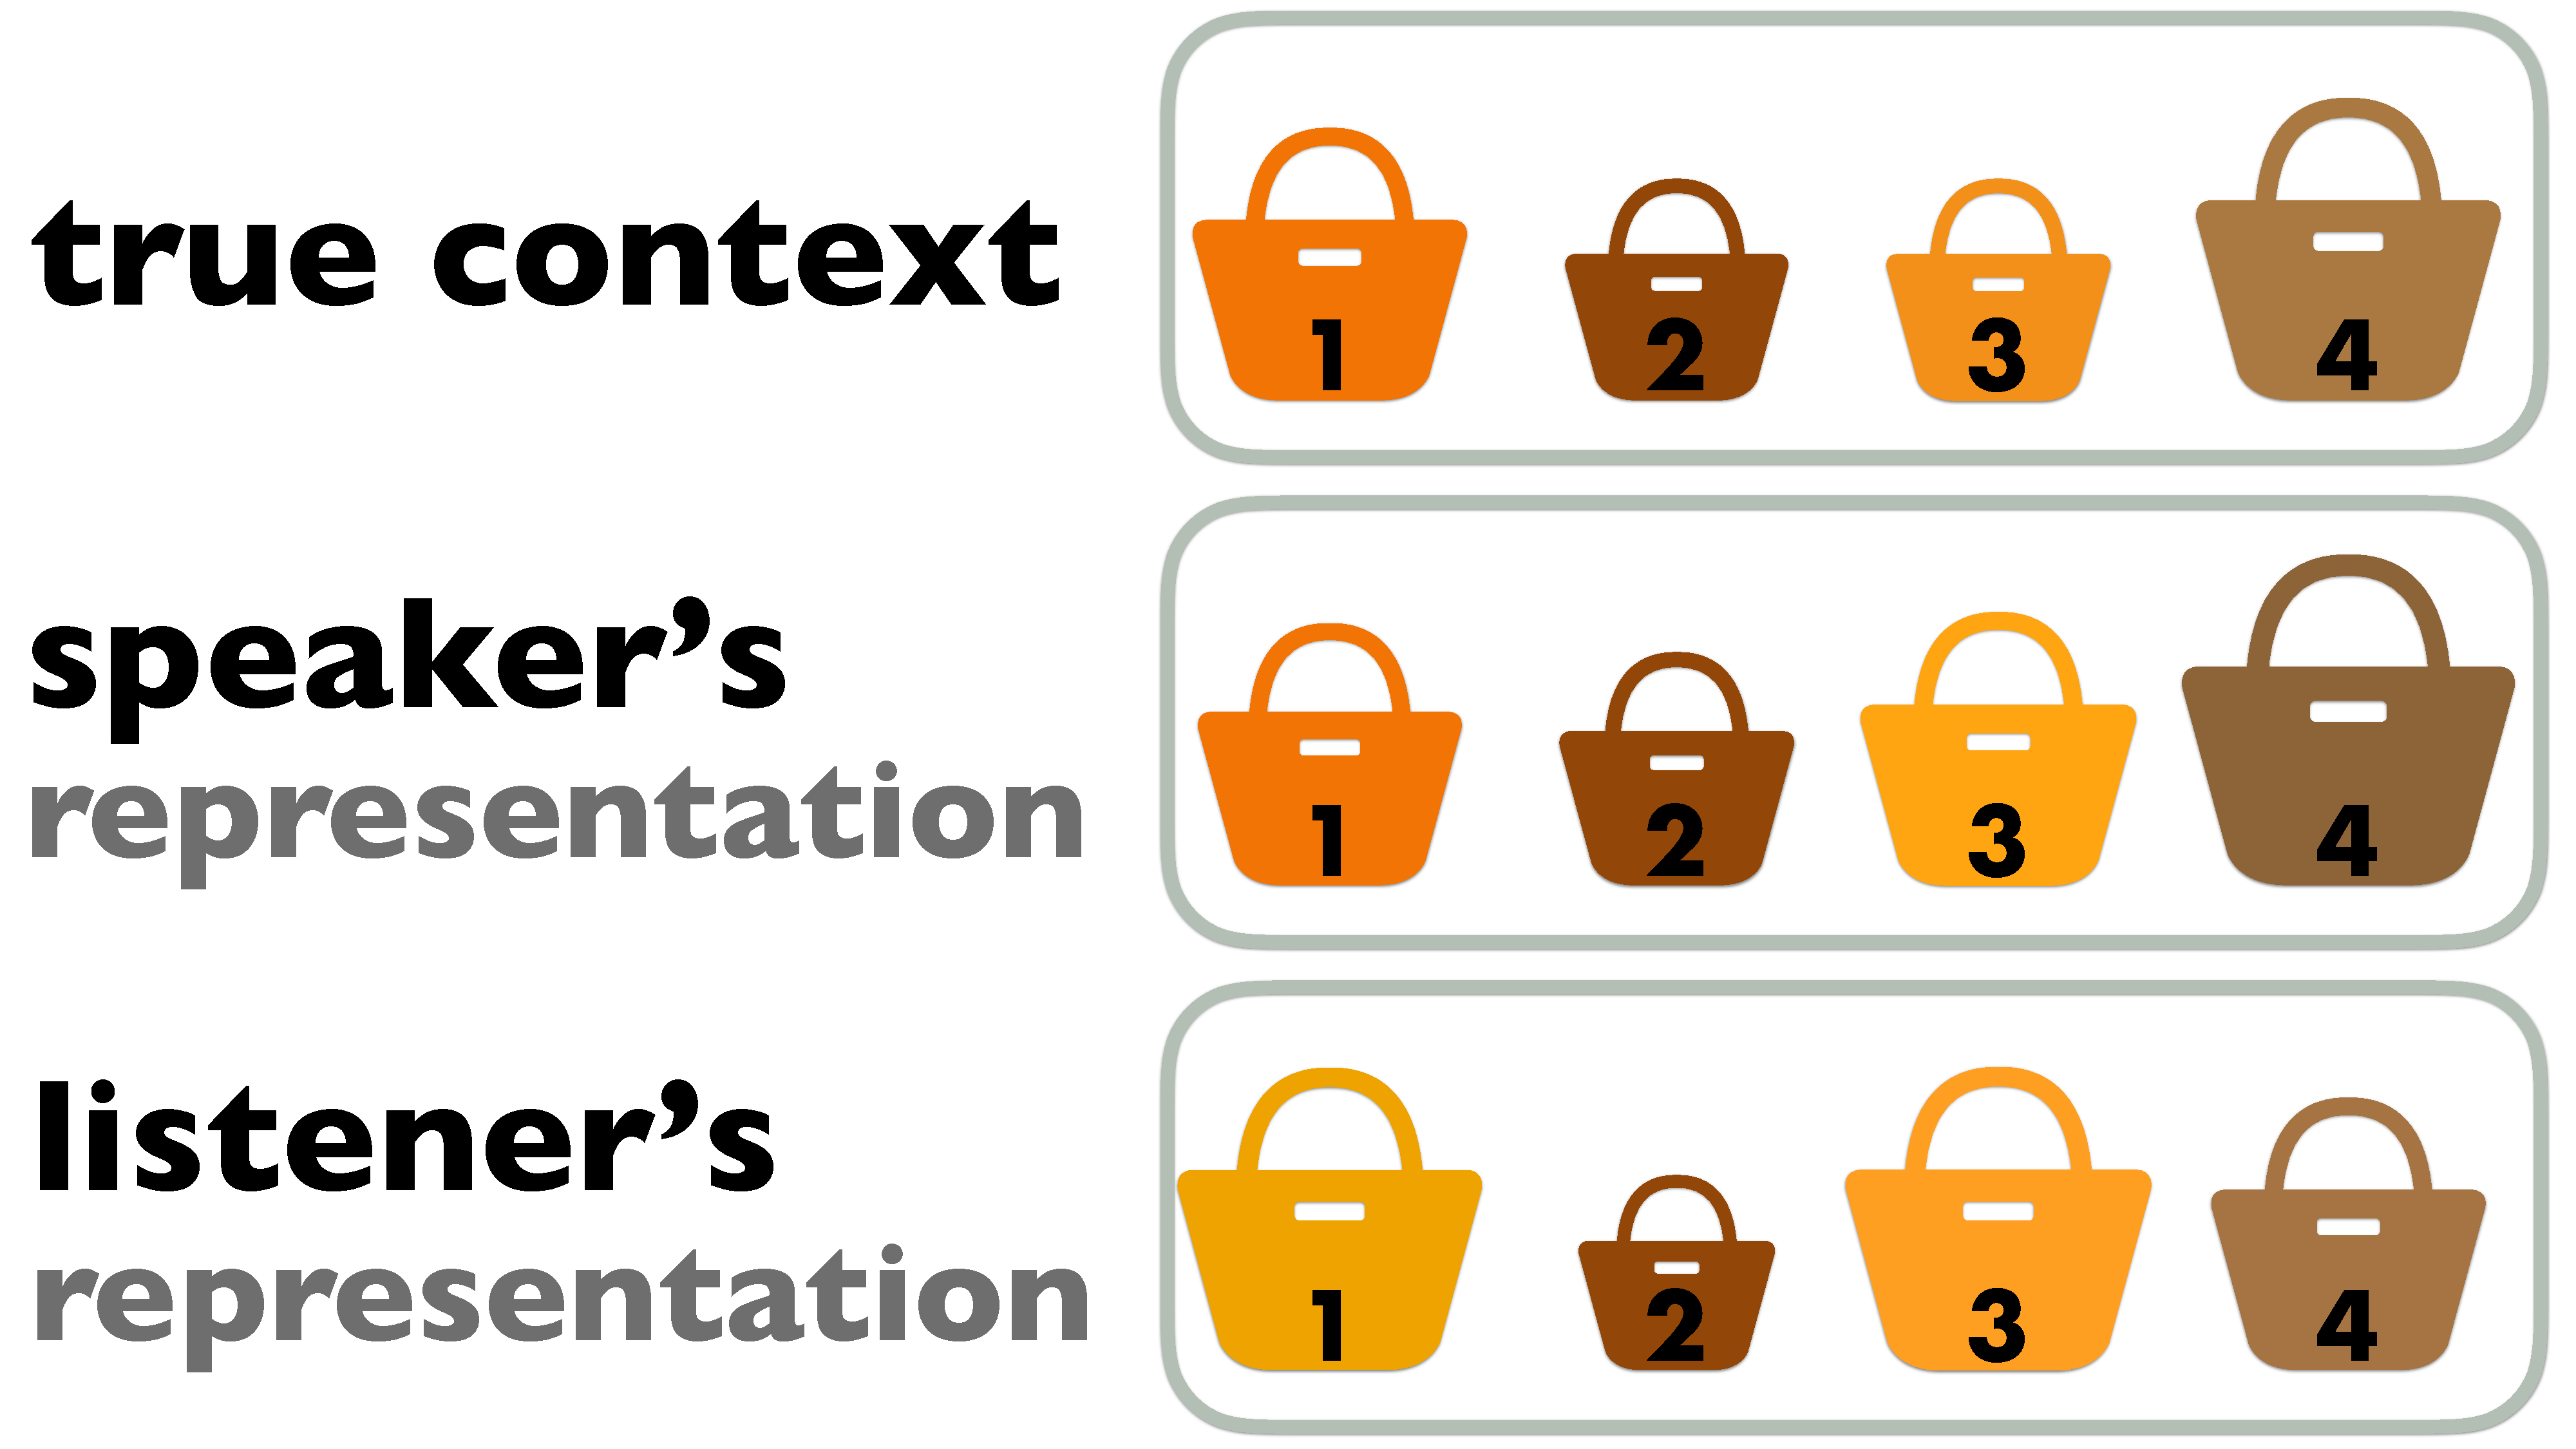
\includegraphics[width=\linewidth]{model_picture.pdf} 
  \caption{Illustration of the model}
  \label{fig:ModelIllustration}
\end{figure}

To get this reasoning off the ground, we first need to make some assumptions about the effects of adjective subjectivity on our mental representations---representations that will be relevant to referential communications. Figure~\ref{fig:ModelIllustration} gives a concrete example to illustrate the main idea. Suppose that speaker and listener share access to a context of four bags that differ only with respect to two properties, color and size. Depending on their different perceptual angles, different background knowledge, or differences in previous experiences, speaker and listener might represent the context differently: their impressions of object size and object color could deviate from the ground truth. 

Here is where subjectivity comes in: more subjective properties are more likely to lead to deviation between the ground truth (i.e., the true context) and an agent's representation of the property. Crucially, by deviating from the ground truth, these more subjective properties are also more likely to lead to deviations between two agent representations (e.g., between the speaker's and listener's representations in Figure \ref{fig:ModelIllustration}); these deviations \emph{and our awareness of their potential} are what lead to perceived subjectivity as measured by a faultless disagreement task. Language users are aware that their representations might deviate from each other's, and the potential for deviation is different for different properties. We illustrate this tendency in Figure \ref{fig:ModelIllustration}, where the agent representations of size deviate more from the ground truth than their representation of color.

We now ask: if the speaker wants to describe a bag that is both big and brown according to her subjective representation of the context, would it be better, on average, to describe it as ``big brown bag'' or ``brown big bag'', knowing that the listener would interpret either phrase from his own subjective perspective? Concretely, suppose the speaker wants to refer to bag 4 in Figure \ref{fig:ModelIllustration}, which is both brown and big from her subjective point of view. If the listener hears ``big brown bag'', he tries to find the speaker-intended referent by incrementally restricting the set of possible referents according to the expression's syntactic structure. The listener therefore first considers all of the bags that are brown (given the comparison set of bags), and then rules out those that are not big (given the comparison set of brown bags). The process is similar for the phrase ``brown big bag'', but the result might be different since at each step of incremental context-narrowing the comparison class against which the listener evaluates the meaning of ``brown'' and ``big'' could differ. 

This through this process of incremental restriction for the example from Figure~\ref{fig:ModelIllustration}, the phrase ``brown bag'' would make the listener exclude bags 1 and 3 (on the assumption of the semantics of \citeA{schmidtetal2009} introduced above with, say, $k = 50\%$). From the remaining bags (2 and 4), only 4 is in the top 50\% along the range of size in this context set. So, the interpretation of ``big brown bag'' is successful; the listener recovers the speaker-intended referent uniquely. In contrast, for the expression ``brown big bag'', the listener first looks at the bags that count as big, which plausibly would rule out bag 2. Among the remaining bags 1, 3 and 4, bag 3 is clearly not brown. For the sake of this informal example, assume that the listener therefore considers both bags 1 and 4 as possible referents when hearing ``brown big bag''. The chance of referential success (i.e., choosing bag 4)---neglecting salience or other factors---would be $\nicefrac{1}{2}$, lower than the certain communicative success when interpreting ``big brown bag''.


\section{Computing average communicative success}

We use a Monte Carlo simulation to estimate the difference in expected referential success between phrases ``big brown bag'' and ``brown big bag'' when averaging over many different contexts with different numbers of objects and varying degrees of subjectivity for the properties involved. A single run of the Monte Carlo simulation proceeds as follows:

\begin{enumerate}
\item We begin by sampling a number $n$ of bags in the current conversational context (more generally: the number of objects of which the modified noun is true); $n$ gets sampled uniformly at random from 4 to 20. 
\item For each object $o$, we sample the degree to which $o$ is brown and the degree to which it is big. These samples are obtained from independent draws from a standard normal distribution. This sampling yields a representation of the \emph{actual context} $C$ as an $n \times 2$ matrix of feature values for the $n$ objects. The probability of sampling context $C$ for fixed $n$ is
  \begin{align*}
  P(C \mid n) = \prod_{i=1}^n \prod_{j=1}^2 \mathcal{N}(C_{ij} \mid \mu = 0, \sigma = 1)\,.
  \end{align*}
\item Agent $X$'s (speaker's or listener's) subjective representation $C^X$ of $C$ is derived from $C$ by assuming normally distributed noise around the property degrees in $C$, with a fixed standard deviation for each adjective. The probability of obtaining a subjective representation $C^X$ from actual context $C$ is
  \begin{align*}
P(C^X \mid C) = \prod_{i=1}^n \prod_{j=1}^2 \mathcal{N}(C_{ij}^X \mid \mu = C_{ij}, \sigma = \sigma_j)\,.
  \end{align*}
The standard deviations $\sigma_{1,2}$ are obtained by sampling two numbers uniformly from the interval XYZ \mf{fill me!} and assigning the higher number to the more subjective adjective (``tall''), the lower to the less subjective adjective (``brown'').
\item A \emph{semantic threshold} $\theta \sim \mathcal{U}(0,1)$ is sampled uniformly at random from the unit interval. By the semantics of \citeA{schmidtetal2009}, the denotation $\sem{adj\textsubscript{j}}^{C}$ of adjective $j \in \{1,2\}$ relative to some context $C$ (actual or subjective; possibly further restricted by previous adjectival modification) is the set of all objects $i$ such that $C_{ij} > \max_{i'}C_{i'j} - \theta \cdot (\max_{i'}C_{i'j} - \min_{i'}C_{i'j})$. The denotation of the phrase ``[adj\textsubscript{i} [adj\textsubscript{j}]]'' is:
  \begin{align*}
   \den{\text{[adj\textsubscript{i} [adj\textsubscript{j}]]}}^{C^X} & = \den{\text{adj}_i}^{\den{\text{adj}_j}^{C^X}} 
  \end{align*}
  \mf{Should some of this go into the previous section on semantics? --- I tend to say yes.} \gcs{hmm.. probably. I've left a placeholder above.}
\item We then sample the \emph{speaker-intended referent object} $i^*$ randomly from the set $\den{\text{adj}_1}^{C^S} \cap \den{\text{adj}_2}^{C^S}$ (i.e., an object that is both brown and big from the point of view of the speaker). If there is no such object, the run is discarded.
\item If the listener's interpretation of the phrase ``[adj\textsubscript{i} [adj\textsubscript{j}]]'' from his subjective point of view is $I = \den{\text{[adj\textsubscript{i} [adj\textsubscript{j}]]}}^{C^L}$, the probability of recovering the intended referent is $|I|^{-1}$ if $i^* \in I$ and 0 otherwise. We record the probability of recovery for both adjective orders and evaluate their distribution over all samples obtained in this way.
\end{enumerate}

\section{Results}

The results are insane!

\bigskip
\bigskip
\bigskip

\mf{maybe recycle the following for the discussion? as in: critical assumptions that could be challenged? \dots}

The model implements a number of assumptions. The most important ones, from a theoretical point of view, are these. First, we assume that the more subjective a property is, the bigger the average/expected inter-subjective differences in context representations are. In other words, we operationalize the subjectivity of property $A$ here as the degree to which, on average, listeners and speakers will have diverging (meaning-relevant) representations of the same object's property $A$. Second, we assume that adjectival modification is, at least sometimes, incrementally intersective, i.e., it follows the syntactic structure and not the surface order. Finally, we assume that adjectives have, at least sometimes, a reading that is entirely or in part determined by the local context only, so that we would interpret the meaning of ``big''  in the phrase ``big brown bag'' as ``big for the brown bags''.

\bigskip





\bibliographystyle{apacite}
\setlength{\bibleftmargin}{.125in}
\setlength{\bibindent}{-\bibleftmargin}

\bibliography{adjOrder}

\end{document}

